\begin{figure}
  \begin{tabular}{cc}
    \begin{minipage}{0.5\hsize}
      \includegraphics[width=6cm]{../pic/Dron/pimSp_data.eps}
    \end{minipage}
    \begin{minipage}{0.5\hsize}
      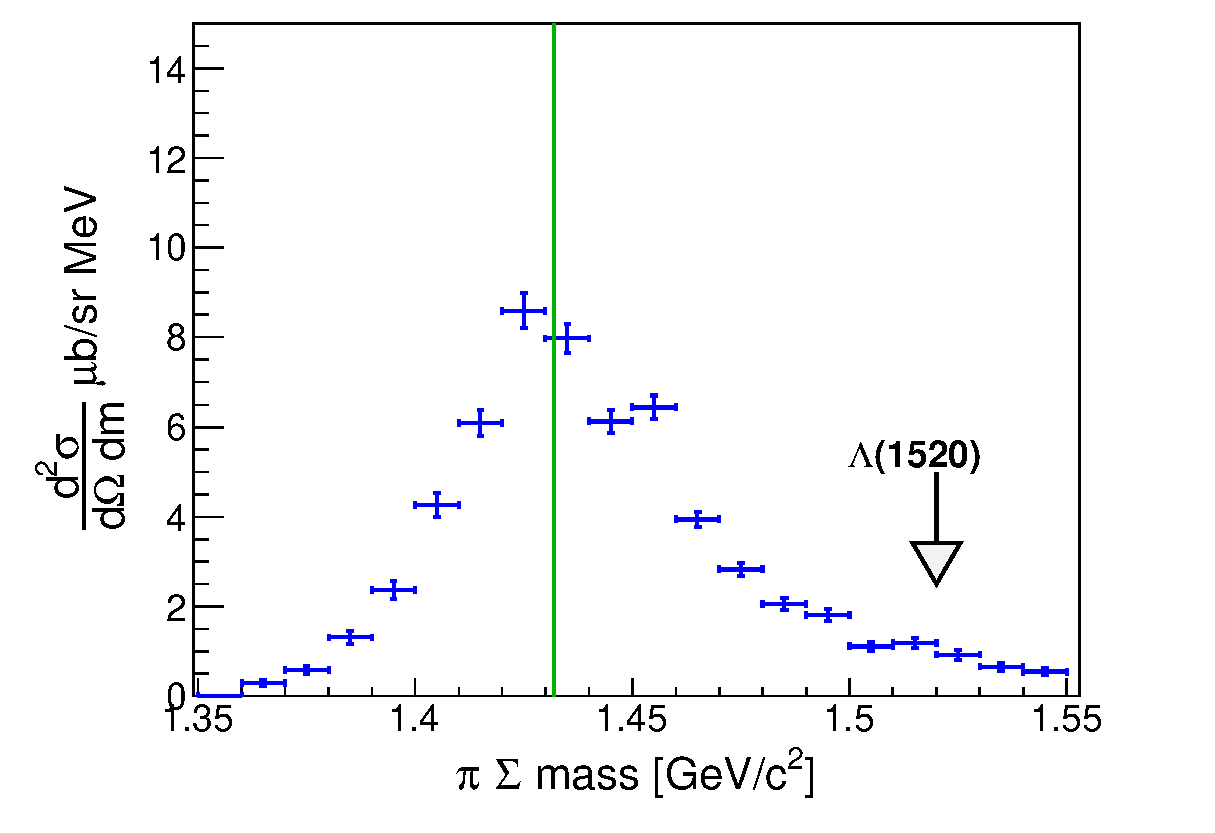
\includegraphics[width=6cm]{../pic/Dron/pipSm_data.eps}
    \end{minipage}
  \end{tabular}
  
  \begin{tabular}{cc}
    \begin{minipage}{0.5\hsize}
      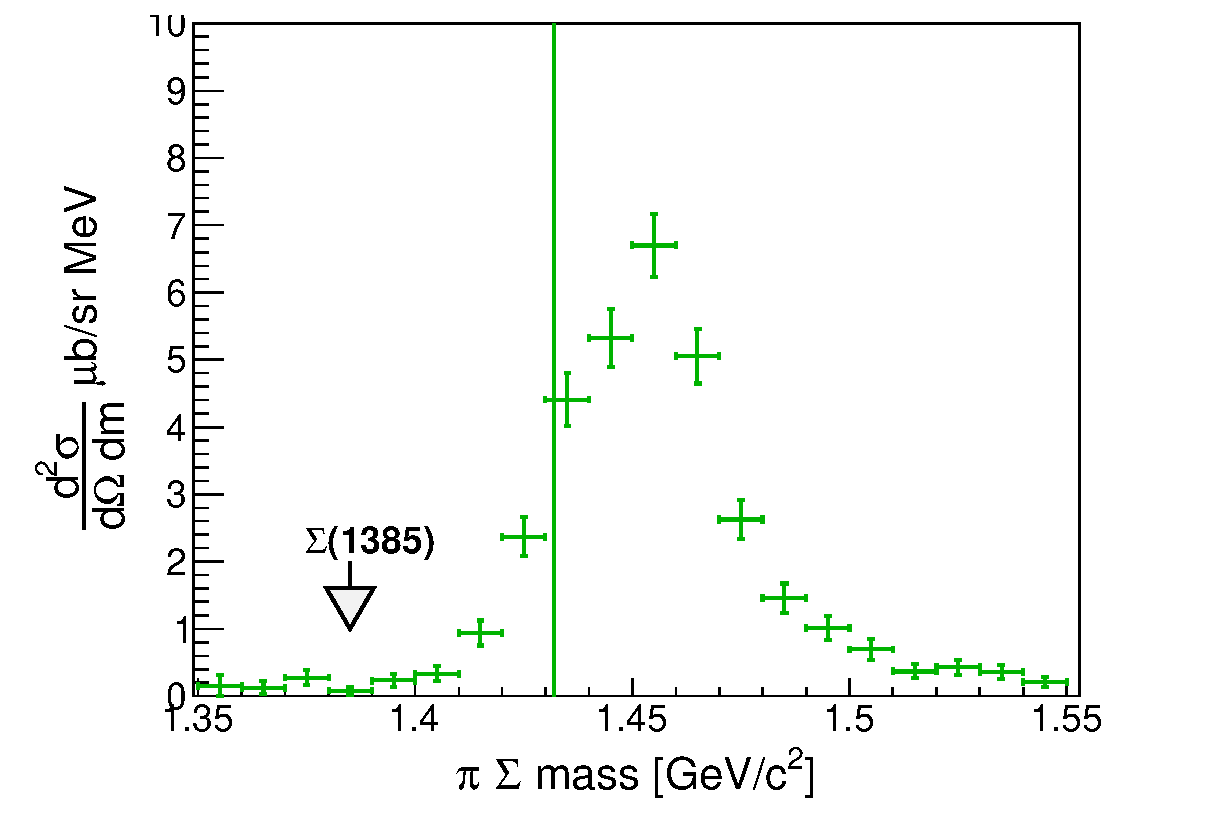
\includegraphics[width=6cm]{../pic/discussion/pimS0_data.eps}
    \end{minipage}
    \begin{minipage}{0.5\hsize}
      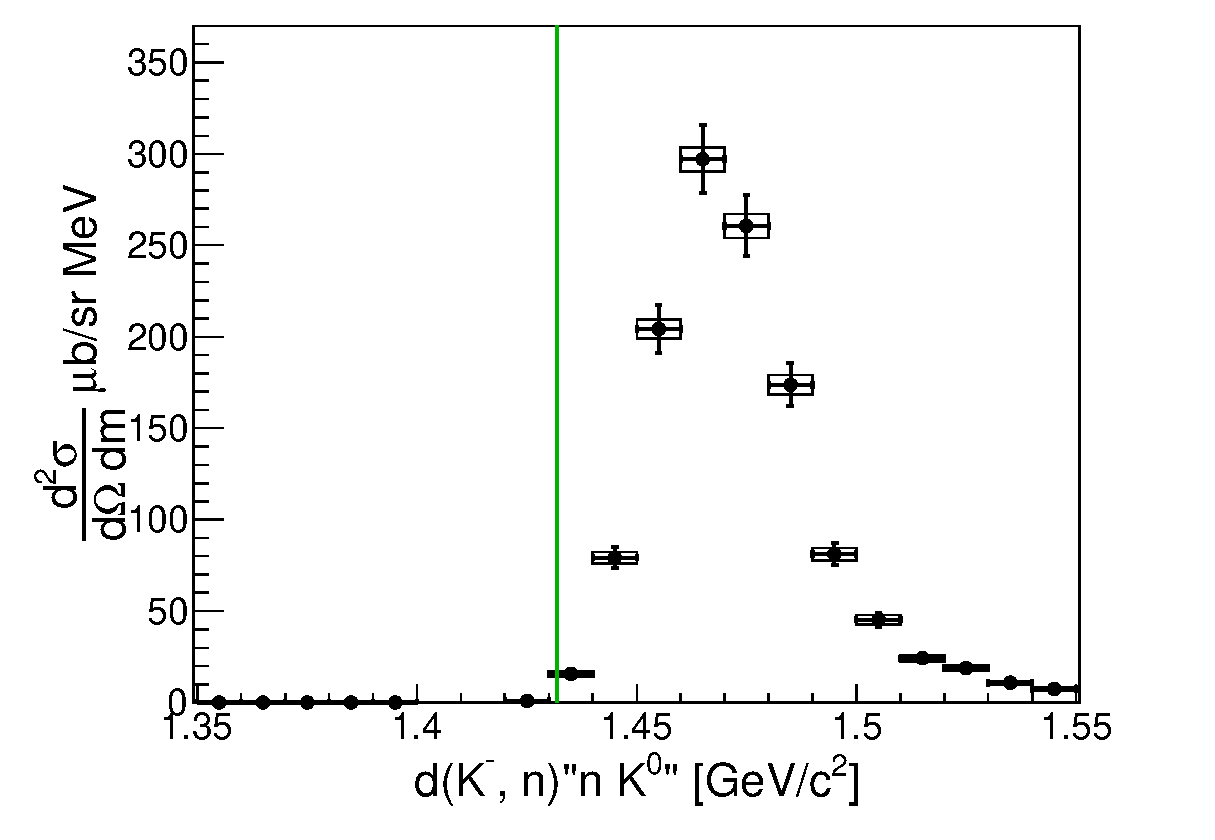
\includegraphics[width=6cm]{../pic/Run78/QE/K0_CS2.eps}
    \end{minipage}
  \end{tabular}
  \caption{
    These figures show obtained spectra.
    \dKNpimSp, \dKNpipSm, \dKPpimSz and $d(K^-, n)"n K^0"$ indicate in left top, right top, left bottom and right bottom, respectively.
    Green vertical line represents $\bar{K}N$ threshold.
    Arrows indicates $\Sigma(1385)$ and $\Lambda(1520)$ position in each figures.
  }
  \label{fig:obtained}
\end{figure}
